\ifdefined\included
\else
\setcounter{chapter}{6} %% Numéro du chapitre précédent ;)
\dominitoc
\faketableofcontents
\fi

\chapter{Challenging Robot Navigation Systems by Simulating Intelligent Human: InHuS}
\chaptermark{Challenging Robot Navigation Systems by Simulating Intelligent Human: InHuS}
\label{chap:7}
\minitoc

\section{Introduction}
Vers simulation humain intelligent pour benchmarker planner robot (nav + tache)

An interactive simulator for user study is useful but not automated

InHuS:
ère du digital twin : 1er pas vers ça, un peu générique, fait pour nav mais pourrait aller plus loin
A mettre dans un chapitre "a part"

Objectives - Current challenges in testing ha nav

\section{Related work}

\textbf{TODO: Cite all the ones in zotero, and from paper}

\section{Description}
 
The InHuS System%
\footnote{https://github.com/AnthonyFavier/InHuS\_Social\_Navigation}
works along with a human operator, a chosen simulator, and the challenged robot controller as depicted in Fig.~\ref{fig:overview}. The system is mainly implemented using ROS. The InHuS  System is three-sided. First, the system comes with a high-level interface called Boss that helps to manage the simulated agents. Secondly, there is the main part which is the intelligent human avatar controller itself, called InHuS.
Finally, a GUI provides an interactive visualization of the data and metrics computed by InHuS during execution that can help to evaluate interactions. We present below some details for each component.

\begin{figure}[ht]
    \centering
    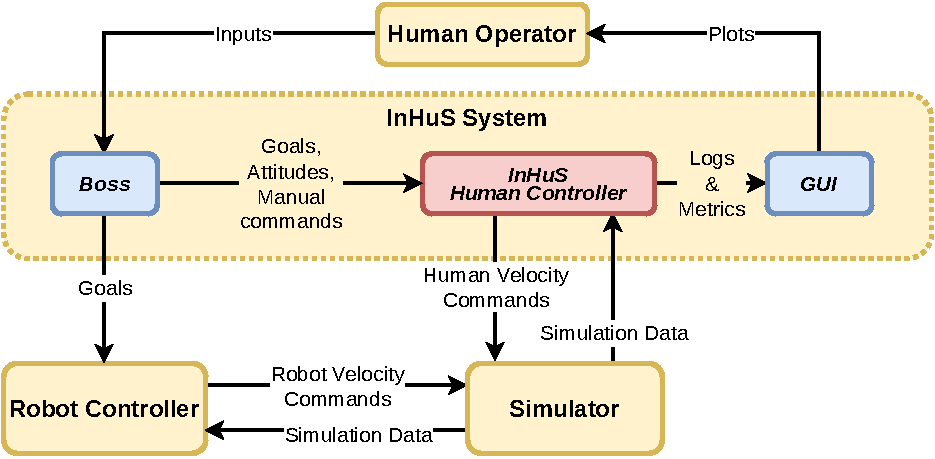
\includegraphics[width=0.7\linewidth]{Chapter7/Inhus.drawio.pdf}
    \caption{
    The InHuS System interacts with three external systems: the simulator, the robot controller, and a human operator. Our system is separated into three parts: the Boss high-level interface gathering inputs from the human operator, InHuS which is the actual human controller, and a GUI to plot the metrics and other data produced.
    }
    \label{fig:overview}
    \vspace{-0.8cm}
\end{figure}

\subsection{Boss}
For the human operator to easily control the simulated agents and run repeatable scenarios, we provide a simple graphical user interface component called Boss. Predefined or manually entered goals can be sent to the human, the robot, or both. Goals are by default considered as ``Pose goals'' that only require one navigation action to be achieved. However, the human agent (only) can handle ``Compound goals'' that need a specified sequence of navigation and waiting for actions to be achieved. This type of compound goal is useful to emulate more complex activities. For example, ``Make coffee'' could be described as a sequence of three actions: nav(coffeeMachine), wait(15$s$), nav(myOffice).

The Boss allows defining scenarios with start positions and goals for each agent to repeatedly generate the same situation. 
Running a scenario consists of first sending each agent to their respective starting position. Then, the corresponding goals are sent to the human and the robot.
A delay can be specified while starting the scenario to delay either the robot's or the human's goal. This is very useful to adjust the timing of a specific situation or conflict. The Boss can also put an agent in ``endless'' mode where the agent continuously gets a new goal from a given list after completing one. 

Each navigation action can specify a radius for the ``Pose goal'', within which a new ``Pose goal'' is randomly sampled. This mechanism adds randomness to the execution and diversifies the situations encountered, especially in the ``endless'' mode. Setting the radius to zero disables the randomization and selects the given goal.

All the goals, scenarios, and endless goal sequences are defined using an XML format. Hence, defining new goals or scenarios is straightforward. There is an XML goal file associated with each map/environment. Thus, it is easy to switch between environments since the corresponding goal file is automatically loaded.


\subsection{InHuS}

\begin{figure}[b]
    \centering
    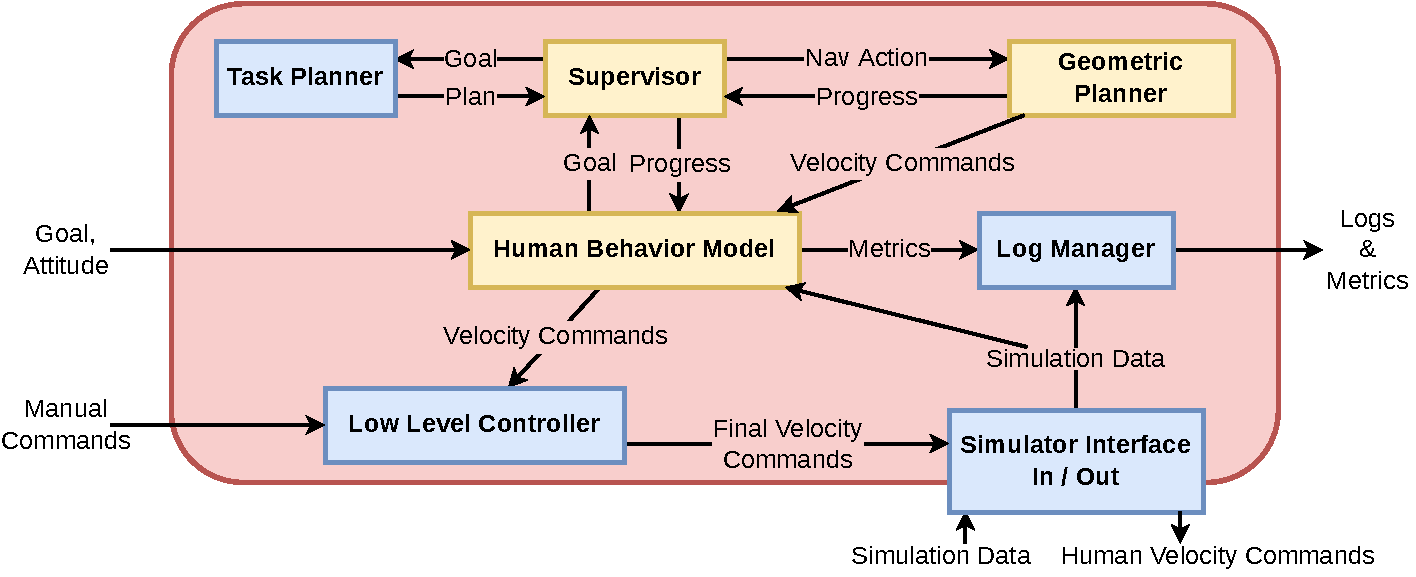
\includegraphics[height=120pt]{Chapter7/inhus_2.pdf}
    \caption{
    The human controller InHuS with its components and subsystems. 
    }
    \label{fig:inhus_only}
    \vspace{-1cm}
\end{figure}

The macro component InHuS is mainly in charge of controlling the avatar and generating rational behaviors. InHuS itself is made of several components as depicted in Fig.~\ref{fig:inhus_only}. However, three components, namely HumanBehaviorModel, Supervisor, and GeometricPlanner, constitute the major functional part of InHuS. We discuss each of these major components in detail.


\subsubsection{HumanBehaviorModel:}

The HumanBehaviorModel is responsible for most of the rational behavior of the agent. The first role of this component is to manage the goals. Goals can either be received from the Boss component or generated by the HumanBehaviorModel using the same XML file as the Boss. When a goal is selected, it is sent to the Supervisor for execution. 

This component is also responsible for detecting and handling navigation conflicts. Currently, the kind of navigation conflict handled by InHuS is path blockage (e.g. another agent standing in a doorway). While the human agent is navigating, a path to the goal is calculated at regular intervals using Dijkstra's algorithm, and its length is tracked to detect such conflicts. If the tracked path length increases significantly or the path ceases to exist, it could mean that another agent is blocking either the only possible way or the shortest way. When such situations are detected, the plan execution is temporarily suspended, and the agent performs an approach action to get close to the blocking location. This shows the agent's intention to move in a specific direction and might induce the blocking agent to react and clear the way.
Eventually, once the avatar is at a specified distance of the blocking location, here set to \SI{1.5}{\metre}, the agent stops its approach and actively waits for the path to be cleared.

To generate a lot of different and specific situations, we created what we call \textit{Attitudes}. They are operating modes affecting both goal decisions and reactions toward the other agents. One can activate them through the Boss to generate diversified behaviors of the agent. Some of the \textit{Attitudes} currently implemented in InHuS consist of: 1) randomly picking a new goal, like someone suddenly changing their mind, 2) harassing the robot by constantly going in front of it, like a child would do \cite{nomura2016children}, and 3) stopping close to the robot and looking at it for a few seconds before resuming its goal which emulates a curious behavior. 

The final purpose of this component is to build the perception of the human agent based on the map and information about the other agents from the simulator. We build the perception by directly accessing the simulation data rather than adding simulated sensors to the human avatar. Using this perception, we compute the visibility of the human agent and then update the human's knowledge about the robot's position and speed.

\subsubsection{Supervisor:}
The Supervisor is a central component as it coordinates different components to execute the plan and achieve the current goal. When the Supervisor receives a goal from the HumanBehaviorModel, it requests the TaskPlanner component a plan to achieve the goal. For now, the plan generation is quite simplistic. For a ``Pose goal'', a plan filled with a single navigation action is generated. For a ``Compound goal'', the sequence of navigation and waiting actions is extracted from the XML goal file and the plan is populated. Despite the simplistic plan generation, this architecture handles complex goals that require several steps to be achieved and emulate human activities.  

The execution of each action of the plan is then supervised by the Supervisor by sending requests to other components. 
When a navigation action needs to be performed, the Supervisor starts by sampling a random position if the given action radius is not zero. Then, it requests the GeometricPlanner to plan for the target position without considering other agents initially. This way, the avatar starts following the shortest path, and we initialize the conflict detection. After this, the system starts to consider the other agents, and the Supervisor periodically requests the HumanBehaviorModel component to check for potential navigation conflicts. The Supervisor can suspend and resume the plan execution at any time, which can be used to resolve the detected conflicts or to generate specific reactions like the \textit{Attitudes}.

\subsubsection{GeometricPlanner:}

The last major component is the GeometricPlanner. This motion planner component receives a target position to reach from the Supervisor and generates velocity commands to make the avatar move. This component defines how the agent moves around and adapts its velocity to the other agents in the scene. Since the system is implemented in ROS, we use the standard ROS navigation stack for the GeometricPlanner.

The planner used in InHuS is a publicly available human-aware navigation planner called CoHAN \cite{singamaneni2021human}. It is built over the ROS navigation stack and uses a local planner based on a modified version of the timed elastic band with human-aware properties. 
We benefit from the high-level decision-making of InHuS and the enhanced local navigation of CoHAN with trajectory predictions. Moreover, CoHAN is highly tunable which helps to generate different agent behaviors. 

\subsection{Logs, metrics and GUI} \label{sec:logs_metrics}

\begin{figure}[!b]
    \centering
    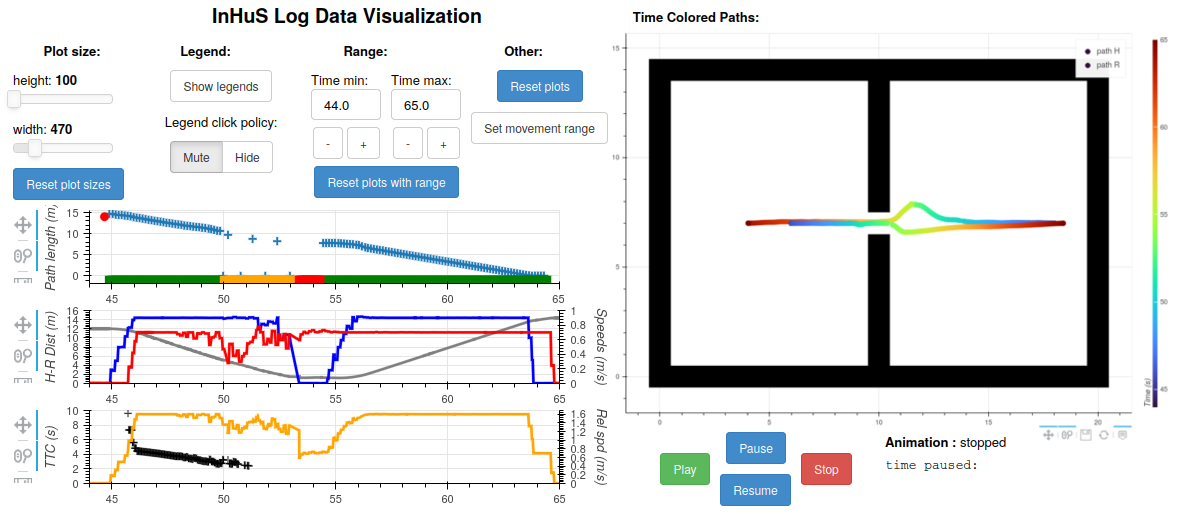
\includegraphics[width=0.8\linewidth]{Chapter7/gui_bis_bis.png}
    \caption{
    Overview of the GUI interface which is organized as follows. On the right side are shown the paths taken by the agents and colored over time. On the left side, several metrics and data produced by InHuS are plotted over time on graphs. Additional widgets help to configure the plots. 
    }
    \label{fig:gui}
\end{figure}

The InHuS system logs the execution data like the positions and speeds of the agents along with some computed metrics. All the logged data is sent to the GUI component, which generates interactive plots. These plots can help evaluate the interaction and thus the performance of the given robot controller. The snapshot of the GUI shown in Fig.~\ref{fig:gui} shows two kinds of visualizations. On the right side, there is a colored visualization of the paths taken by each agent. These paths are colored over time according to a corresponding legend that helps estimate an agent's position at a specific moment. The left side is composed of several plots showing some computed metrics over time. The first plot is about conflict detection and solving. It shows the length of the path to the goal computed when checking for conflicts. Without any conflict, the path length should decrease linearly over time. If it's not the case, the avatar has been disturbed during the navigation. This plot also shows the conflict state of the agent: Nominal (no conflict), Approach (conflict detected), Blocked (stopped and waiting). The subsequent plots show over time the speeds of each agent, their relative speed, the distance separating them, 
and a metric called time to collision (TTC). This metric estimates the time remaining before the agents collide with their current velocities. We can argue that TTC corresponds to a ``threat feeling'' since a low TTC value corresponds to a high threat of collision. Hence, social robots should be tuned to not exceed a minimum TTC value to make humans more comfortable.

\section{Main results}
able to numerically identify the HA behavior of CoHAN w/r SMB)


In this section, we show some results through a set of experiments to highlight how our system can help challenge human-aware robot navigation systems. First, we discuss the limits of reactive-only systems to strengthen the need for rational avatars. 
Then, we present how our system effectively challenges robot navigation systems and we interpret the corresponding plots.
Next, we show how the InHuS System can compare the human-aware performances of two different robot controllers.
Finally, we present additional experiments showing the diverse behaviors that can be produced using the \textit{Attitudes}, and how ``long runs'' can benefit the development of a robot controller.

\subsection{Limits of reactive-only agents}
\label{sec:pedsim_compare}
Most of the current human agent simulations used by the social navigation community rely either on the social force model or ORCA. In order to highlight the limitations of such approaches, we present results obtained with a PedSim\_ROS (or simply PedSim) agent. PedSim is a pedestrian simulator that uses the social force model. It is very efficient for generating crowds to test robot navigation. However, at the individual level, the simulated agents are purely reactive and have no decisional abilities like most pedestrian simulators. 

\begin{figure}
    \centering
    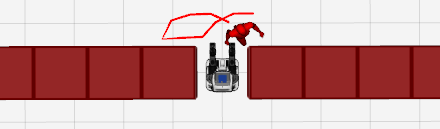
\includegraphics[width=0.4\linewidth]{Chapter7/pedsim_blocked.png}
    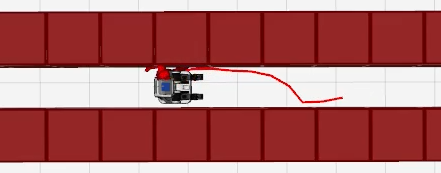
\includegraphics[width=0.4\linewidth]{Chapter7/pedsim_narrow_2.png}
    \caption{
    In the doorway scenario (left), the reactive-only (Pedsim) agent never stops moving while trying to go through the robot even though its path is blocked. 
    In the narrow corridor scenario (right), the agent squeezes itself between the wall and the robot colliding with both. 
    }
    \label{fig:limits_reactive}
    \vspace{-0.3cm}
\end{figure}

Consider the doorway scene shown in the left part of Fig.~\ref{fig:limits_reactive}. Both agents have to cross a narrow opening. Here, the robot is blocking the way that the human agent intends to cross. The PedSim agent approaches the robot and tries to push itself through, but it fails due to a very high value of social force. The agent never stops moving and tends to go right or left along the wall before wiggling again just in front of the robot. 
This confusing behavior can make the agent's intentions unclear to the robot planner. 
The narrow corridor scenario, shown in the right part of Fig.~\ref{fig:limits_reactive}, also exposes some limits. In this scene, there is not enough space for the agents to cross each other,  and the only solution is for one of them to back off. Here the path is blocked by the static robot. The PedSim agent slowly gets closer and closer to the robot before squeezing itself between the wall and the robot. For some reason here the social forces allowed the agent to pass, unlike the previous example. It highlights that the PedSim agent doesn't use a defined hitbox or footprint for the agent and relies only on repulsive social forces to prevent collisions. This lack of defined collision shapes makes the agent temporarily pass through the walls and other agents. As a consequence, it breaks many intricate scenarios where a rational decision should be taken and results in unrealistic situations. Despite being efficient for large spaces or crowds, based on the above observation, we can state that in intricate scenarios such approaches can lead to confusing and even unrealistic behaviors.  

\subsection{Interpretation of plots with human-aware planner}

The InHuS System is able to generate challenging situations 
and associated logs to allow further evaluation.
Here, we present one such conflict and a detailed interpretation of the corresponding plots. The plots were produced while challenging the CoHAN system in the doorway scenario.

\begin{figure}
    \centering
    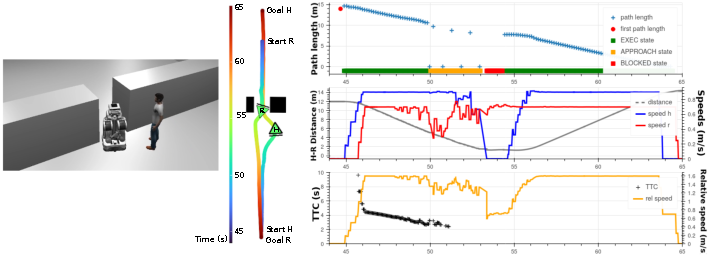
\includegraphics[width=1.0\linewidth]{Chapter7/test.pdf}
    
    \caption{
    A condensed view of the InHuS GUI and MORSE simulator for the doorway scenario with a robot running the CoHAN planner. Several plots depict the detection and resolution of the conflict created. 
    }
    \label{fig:cohan_passage_block}
    \vspace{-0.3cm}
\end{figure}


The robot starts closer to the opening and enters the doorway first. The execution can be analyzed with the metric plots and the time-colored paths of the agents in Fig.~\ref{fig:cohan_passage_block}. We notice that the robot's speed (red line on the second graph) goes down around \SI{50}{\second} as it is entering the doorway and creating a conflict. The conflict is detected by InHuS (zero path length = no path), and the agent switches to the approach state (green to the yellow line on the first graph).
The non-zero path length in the approach state corresponds to how the approach is performed. In order to keep moving despite the blocked path, the GeometricPlanner is requested at a defined frequency to plan without considering the robot (all non-zero path length). In between these requests, to check if the path is still blocked, the conflict detection plans while considering the robot (zero path length). When the avatar is at a predefined distance from the blocking robot around \SI{53}{\second}, it switches to the blocked state (red line) to stop and wait for the path to be cleared. Further, the time-colored paths show that the GeometricPlanner made the avatar move aside while approaching to avoid blocking the robot. As a result, the agents were no longer moving towards each other, and thus, there was no longer any collision threat (no TTC values). When there is no more collision threat, around \SI{51}{\second}, the robot's speed starts to increase again. Such behavior is a good sign of human-aware properties and might increase human comfort.

From the plots produced by our system, a lot of useful information can be extracted for improving or evaluating the social robot planner's performance like a) finding ways to decrease the blocked state time for the human, b) maintaining a particular threshold for TTC, c) slowing down near the human, or waiting for the human to cross the door without blocking.


\subsection{Quantitative comparison between two robot controllers}

Our system can be used to run similar scenarios repetitively to produce robust metric values. These values can help to evaluate the human-aware performances of a given robot controller. To show this, we present a comparison between two different robot controllers. The first one is again the CoHAN system, and the second one is the Simple Move Base (or SMB). It uses the \textit{teb\_local\_planner} and the ROS navigation stack with default parameters. We just add an additional process to consider the human agent as a static obstacle to avoid it, so it is not human-aware. Therefore, we should be able to notice a clear difference through the metrics computed by our system. For this comparison, we used three different scenarios: 1) The doorway scenario where the agents have to cross a narrow opening, 2) the corridor scenario where the agents cross each other with just enough space, and 3) the open space where they cross each other without any environmental constraints. We performed 10 repetitions of each scenario for each robot controller. For each set of 10 repetitions, we extracted the mean values of three different metrics and presented them in Table~\ref{tab:compare_robots}. The metrics are the following. First, the time to goal (TTG) is the time taken by the avatar to reach its goal. Second, the minimum distance between the robot and the human (Min HRDist). And, the minimum time to collision (TTC). Intuitively, we want the TTG to be as small as possible, the minimum HRDist to be as high as possible, and since a low TTC value represents a collision threat, we want the min TTC to be as high as possible. 

\begin{table}
\vspace{-0.2cm}
    \caption{Mean values of three InHuS metrics over 10 repetitions in three different scenarios and with two different robot controllers. Bold values indicate when the corresponding robot controller has better performance than the other.}
    \label{tab:compare_robots}
    \centering
    \begin{tabular}{|c|c|c|c|c|c|c|}
    \hline
     & \multicolumn{3}{c|}{CoHAN} & \multicolumn{3}{c|}{SMB}\\
    \cline{2-7}
    Experiment & \textit{TTG}$(s)$ & \textit{Min Dist}$(m)$&  \textit{Min TTC}$(s)$ 
    & \textit{TTG}$(s)$ & \textit{Min Dist}$(m)$ & \textit{Min TTC}$(s)$\\
    \hline
    \textit{Doorway} & 18.38 & \textbf{2.32} & \textbf{1.33} & \textbf{18.26} & 2.23 & 1.16\\
    \hline
    \textit{Corridor} & \textbf{16.34} & \textbf{2.06} & \textbf{1.03} & 17.05 & 1.59 & 0.81\\
    \hline
    \textit{Open space} & \textbf{9.55} & \textbf{2.52} & \textbf{1.61} & 11.01 & 2.34 & 1.18\\
    \hline
    \end{tabular}
\vspace{-0.3cm}  
\end{table}

At first glance, we see in Table~\ref{tab:compare_robots} that almost all CoHAN values are better than SMB values. Due to the nature of the doorway environment, the execution of the scenario is quite constrained which explains why the values are not too different between the two controllers. However, we notice anyway that, compared to SMB, the CoHAN planner tends to keep a greater distance between the agents and a greater TTC (lower threat of collision). The time to goal of CoHAN is slightly higher because the robot slows down when crossing and moving in the direction of the human. Thus, it is the price to pay in this scenario to maintain adequate TTC values.

In the corridor scenario, The SMB robot tends to wait until the last moment to move aside, which is threatening. On the other hand, the CoHAN robot proactively moves to one side of the corridor. As a consequence, it leaves more space for humans and reduces the threat of collision, which is visible in the obtained values. Also, this pro-activity has the effect of smoothing the trajectory of the avatar, which makes this last one reach its goal faster.

Finally, the open space scenario is a bit similar to the previous one. The SMB robot waits until the last moment to avoid the human, which puts the load of the avoidance maneuver on the human. As a result, 
the human has to move aside which extends the duration to reach the goal. Also, due to the same behavior, the SMB robot is on average closer to the avatar and more threatening. Since the CoHAN robot moved again aside early, its metric values are noticeably better than SMB.

In summary, the human-aware behavior of the CoHAN controller was captured through significant value differences in the computed metrics compared to a non-human-aware robot controller. This implies that our system can help evaluate and compare human-aware robot controllers.

\subsection{Generating different behaviors with Attitudes}

\begin{figure}
    \centering
    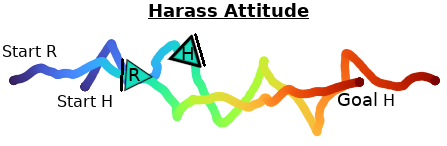
\includegraphics[width=0.45\linewidth]{Chapter7/harass_colored_path_bis.png}
    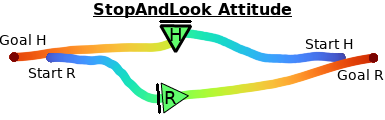
\includegraphics[width=0.45\linewidth]{Chapter7/stoplook_colored_path_bis.png}
    \caption{
    Behaviors obtained by activating the \textit{Harass} and \textit{StopAndLook Attitudes}. 
    With \textit{Harass}, the human is always in front of the robot.
    With \textit{StopAndLook}, when close to the robot, the human stops to look at it for a few seconds.
    }
    \label{fig:attitudes}
    \vspace{-0.3cm}
\end{figure}

By activating \textit{Attitudes}, InHuS is capable of producing more complex behaviors to diversify the conflicts and challenges imposed on the robot.
We present the time-colored paths for the execution of two \textit{Attitudes} : \textit{Harass} and \textit{StopAndLook} in Fig.~\ref{fig:attitudes}. Concerning the \textit{Harass Attitude}, by paying attention to the colors, we see that the human is always in front of the robot that continuously tries to avoid the harassing agent causing erratic movements. The robot should be able to detect such non-cooperative behavior from humans and act accordingly.
On the same figure we see the execution of the \textit{StopAndLook Attitude}. The color discontinuity behind the human marker shows how the human suspended its goal to stop and briefly stare at the robot before moving again. A robot not pro-active enough could be disturbed by the sudden stop of the human, which could be a situation of interest to handle. 


\subsection{Long run scenarios}


\begin{figure}
    \centering
    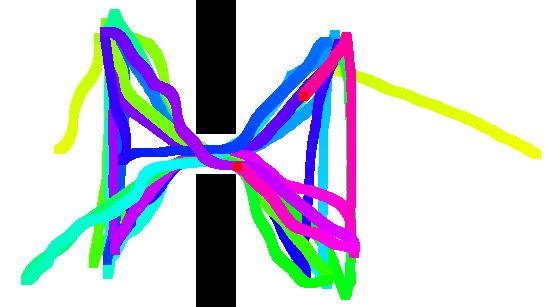
\includegraphics[height=80pt]{Chapter7/TDP_long_run_path.png}
    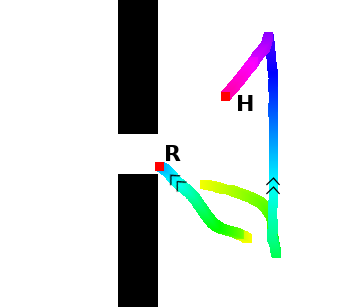
\includegraphics[height=80pt]{Chapter7/TDP_long_run_path_blocked_cropped_final.png}
    \caption{Execution of the long run scenario using the TDP robot planner and InHuS. We see the complete set of time-colored paths on the left. On the right, the same path is cut, around the moment when the robot got stuck in the wall. 
    }
    \label{fig:long_run_block}
    \vspace{-0.3cm}
\end{figure}

The proposed system can help test the stability and robustness of the robot planner by conducting long randomized runs. Indeed, thanks to the Boss component, possibly randomized goals can be sent autonomously to the agents. This can generate unexpected situations and conflicts that can be of interest.
Fig.~\ref{fig:long_run_block} depicts such a test conducted with InHuS and a human-aware robot planner from Kollmitz et. al. \cite{kollmitz_time_2015} here referred to as TDP. The agents were made to endlessly loop over four goal-positions (each with a \SI{1}{\metre} radius) in reverse order to create as many conflicts as possible. After 3 minutes, the robot got stuck in the wall of the doorway, indefinitely blocking the path for the human. In addition to highlighting problematic situations where the robot doesn't act as expected, long runs can expose low-level issues like unexpected crashes or memory leaks.


\section{Extension: IMHuS}

This work has been extended through the help of an intern to the IMHuS framework \cite{hauterville-2022}.

\subsection{Describe}
\subsection{results?}

\section{Discussion and Limitations}
\section{Conclusion}